\documentclass{standalone}
\usepackage{tikz}
\usetikzlibrary{3d}
\begin{document}

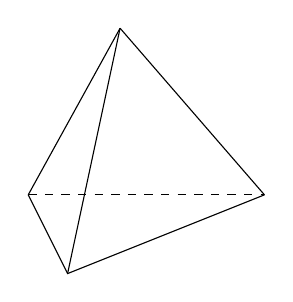
\begin{tikzpicture}[scale = 3]
    % 定义正四面体的顶点坐标
    \coordinate (A) at (0,0,0);%第一个坐标是横的,第二个坐标是往上走,而第三个坐标往纸面外走
    \coordinate (B) at (1,0,0); 
    \coordinate (C) at (0.5, 0,{sqrt(3)/2});
    \coordinate (D) at (0.5,{sqrt(6)/3} , {sqrt(3)/6});

    % 绘制正四面体的边
    \draw (A) -- (C) -- (B);
    \draw[dashed] (A) -- (B);
    \draw (A) -- (D);
    \draw (B) -- (D);
    \draw (C) -- (D);
    % \node[ left] at (A) {$A$};
    % \node[right ] at (B) {$B$};
    % \node[below left] at (C) {$C$};
    % \node[above ] at (D) {$D$};

\end{tikzpicture}

\end{document}


% convert -density 300 正四面体.pdf 正四面体.png